\documentclass[11pt,a4paper]{article}
\usepackage{geometry}
\geometry{margin=0.75in}
\usepackage{amsmath, amssymb, amsfonts}
\usepackage{fontspec}
\setmainfont{Kalpurush}

\usepackage{tikz}
\usetikzlibrary{arrows.meta, angles, quotes, calc}
\usepackage{graphicx}

\title{\textbf{পদার্থবিজ্ঞান ও গণিত: ভেক্টর সমস্যাবলি (Problem Set: Vectors)}}
\author{}
\date{}

\begin{document}
\maketitle

% ----------------------------------------------------------------------
% Question 31
% ----------------------------------------------------------------------
\subsection*{প্রশ্ন ৩১}

কোনো বিন্দুতে $\theta$ কোণে ক্রিয়ারত $\vec{P}$ ও $\vec{Q}$ ভেক্টরের লব্ধি $\vec{R}$। যদি $Q$ এর মান দ্বিগুণ করা হয় তবে লব্ধির মান দ্বিগুণ হয়। আবার $\vec{Q}$ কে বিপরীতমুখী (অর্থাৎ $-\vec{Q}$ দ্বারা প্রতিস্থাপিত) করা হলেও লব্ধির মান $2R$ হয়। $P, Q$ ও $R$ এর মানের অনুপাত নির্ণয় করো।

\smallskip
\textit{[The resultant of two vectors $\vec{P}$ and $\vec{Q}$ acting at a point at an angle $\theta$ is $\vec{R}$. If the magnitude of $Q$ is doubled, the magnitude of the resultant doubles. Again, if $\vec{Q}$ is reversed (i.e., replaced by $-\vec{Q}$), the magnitude of the resultant also becomes $2R$. Find the ratio of the magnitudes of $P, Q,$ and $R$.]}

\vspace{0.3cm}
\begin{center}
\begin{tikzpicture}[scale=0.85, >=Stealth]
    \draw[->, thick, blue] (0,0) -- (4,0) node[right] {$\vec{P}$};
    \draw[->, thick, red] (0,0) -- (60:3) node[above right] {$\vec{Q}$};
    \draw[->, thick, purple] (0,0) -- (3.5,2.6) node[above] {$\vec{R}$};
    \draw[dashed, gray] (4,0) -- (3.5,2.6) -- (60:3);
    \draw[->, thick, dashed, red!60!black] (0,0) -- (240:3) node[below left] {$-\vec{Q}$};
    \draw (0.8,0) arc (0:60:0.8) node[midway, right=2pt] {$\theta$};
\end{tikzpicture}
\end{center}

\textbf{সমাধান:}

ধরি, $\vec{P}$ ও $\vec{Q}$ এর মধ্যবর্তী কোণ $= \alpha$।

১ম ক্ষেত্রে:
$$R^2 = P^2 + Q^2 + 2PQ\cos\alpha \quad \text{--- (i)}$$

২য় ক্ষেত্রে ($Q$ এর মান দ্বিগুণ করা হলে লব্ধি $2R$ হয়):
$$(2R)^2 = P^2 + (2Q)^2 + 2P(2Q)\cos\alpha$$
$$\Rightarrow 4R^2 = P^2 + 4Q^2 + 4PQ\cos\alpha \quad \text{--- (ii)}$$

৩য় ক্ষেত্রে ($Q$ কে বিপরীতমুখী করলে লব্ধি $2R$ হয়):
$$(2R)^2 = P^2 + Q^2 + 2PQ\cos(180^\circ - \alpha)$$
$$\Rightarrow 4R^2 = P^2 + Q^2 - 2PQ\cos\alpha \quad \text{--- (iii)}$$

সমীকরণ (i) এবং (iii) যোগ করে পাই:
$$R^2 + 4R^2 = (P^2 + Q^2 + 2PQ\cos\alpha) + (P^2 + Q^2 - 2PQ\cos\alpha)$$
$$\Rightarrow 5R^2 = 2P^2 + 2Q^2$$
$$\Rightarrow 2P^2 + 2Q^2 - 5R^2 = 0 \quad \text{--- (iv)}$$

সমীকরণ (ii) থেকে $2 \times$ সমীকরণ (i) বিয়োগ করে পাই:
$$4R^2 - 2R^2 = (P^2 + 4Q^2 + 4PQ\cos\alpha) - 2(P^2 + Q^2 + 2PQ\cos\alpha)$$
$$\Rightarrow 2R^2 = -P^2 + 2Q^2$$
$$\Rightarrow P^2 - 2Q^2 + 2R^2 = 0 \quad \text{--- (v)}$$

সমীকরণ (iv) ও (v) হতে বজ্রগুণন (Cross-multiplication) করে পাই:
$$\frac{P^2}{(2)(2) - (-5)(-2)} = \frac{Q^2}{(-5)(1) - (2)(2)} = \frac{R^2}{(2)(-2) - (2)(1)}$$
$$\Rightarrow \frac{P^2}{4 - 10} = \frac{Q^2}{-5 - 4} = \frac{R^2}{-4 - 2}$$
$$\Rightarrow \frac{P^2}{-6} = \frac{Q^2}{-9} = \frac{R^2}{-6}$$
$$\Rightarrow \frac{P^2}{2} = \frac{Q^2}{3} = \frac{R^2}{2}$$

উভয় পক্ষে বর্গমূল করে পাই:
$$P : Q : R = \sqrt{2} : \sqrt{3} : \sqrt{2}$$

\textbf{উত্তর:} $P : Q : R = \sqrt{2} : \sqrt{3} : \sqrt{2}$

\vspace{0.5cm}
\hrule
\vspace{0.5cm}

% ----------------------------------------------------------------------
% Question 32
% ----------------------------------------------------------------------
\subsection*{প্রশ্ন ৩২}

পশ্চিম দিকে $4\text{ km/h}$ বেগে হেঁটে চলা একজন লোকের কাছে মনে হলো বৃষ্টি খাড়া নিচের দিকে পড়ছে। লোকটির বেগ দ্বিগুণ করা হলে তার কাছে মনে হলো বৃষ্টি উল্লম্বের সাথে $30^\circ$ কোণে পড়ছে। বৃষ্টির প্রকৃত বেগের মান ও দিক নির্ণয় করো।

\smallskip
\textit{[To a person walking west at a speed of $4\text{ km/h}$, rain appears to fall vertically downward. If the person's speed is doubled, rain appears to fall at an angle of $30^\circ$ with the vertical. Find the magnitude and direction of the actual velocity of rain.]}

\vspace{0.3cm}
\begin{center}
\begin{tikzpicture}[scale=0.6, >=Stealth]
    \draw[->, gray, thin] (-6,0) -- (3,0) node[right] {East ($+x$)};
    \draw[->, gray, thin] (0,-7.5) -- (0,2) node[above] {Vertical ($+y$)};
    \draw[->, thick, blue] (0,0) -- (-4,0) node[above left] {$\vec{v}_m$};
    \draw[->, thick, red] (0,0) -- (-4,-6.92) node[below left] {$\vec{v}_r$};
    \draw[->, thick, green!50!black] (0,0) -- (0,-6.92) node[right] {$\vec{v}_{rm}$};
    \draw[dashed, gray] (-4,0) -- (-4,-6.92) -- (0,-6.92);
\end{tikzpicture}
\end{center}

\textbf{সমাধান:}

পূর্ব দিককে $+x$ অক্ষ এবং খাড়া উপরের দিককে $+y$ অক্ষ ধরি।
ধরি, বৃষ্টির প্রকৃত বেগ $\vec{v}_r = v_x\hat{i} + v_y\hat{j}$।

১ম ক্ষেত্রে:
লোকের বেগ পশ্চিম দিকে হওয়ায়, $\vec{v}_m = -4\hat{i}\text{ km/h}$।
লোকের সাপেক্ষে বৃষ্টির আপেক্ষিক বেগ:
$$\vec{v}_{rm} = \vec{v}_r - \vec{v}_m = (v_x - (-4))\hat{i} + v_y\hat{j} = (v_x + 4)\hat{i} + v_y\hat{j}$$

শর্তানুসারে, বৃষ্টি খাড়া নিচের দিকে পড়ে। সুতরাং, আপেক্ষিক বেগের অনুভূমিক উপাংশ শূন্য হবে:
$$v_x + 4 = 0 \implies v_x = -4\text{ km/h}$$

২য় ক্ষেত্রে (বেগ দ্বিগুণ করা হলে):
নতুন লোকের বেগ, $\vec{v}_m' = -8\hat{i}\text{ km/h}$।
নতুন আপেক্ষিক বেগ:
$$\vec{v}_{rm}' = \vec{v}_r - \vec{v}_m' = (v_x + 8)\hat{i} + v_y\hat{j} = (-4 + 8)\hat{i} + v_y\hat{j} = 4\hat{i} + v_y\hat{j}$$

শর্তানুসারে, বৃষ্টি উল্লম্বের সাথে $30^\circ$ কোণে পড়ে:
$$\tan 30^\circ = \frac{|\text{Horizontal Component}|}{|\text{Vertical Component}|} = \frac{4}{|v_y|}$$
$$\Rightarrow \frac{1}{\sqrt{3}} = \frac{4}{|v_y|} \implies |v_y| = 4\sqrt{3}\text{ km/h}$$

যেহেতু বৃষ্টি নিচের দিকে পড়ে, তাই $v_y = -4\sqrt{3}\text{ km/h}$।

বৃষ্টির প্রকৃত বেগের মান:
$$|\vec{v}_r| = \sqrt{v_x^2 + v_y^2} = \sqrt{(-4)^2 + (-4\sqrt{3})^2} = \sqrt{16 + 48} = \sqrt{64} = 8\text{ km/h}$$

দিক নির্ণয়:
$$\tan\theta = \frac{|v_x|}{|v_y|} = \frac{4}{4\sqrt{3}} = \frac{1}{\sqrt{3}} \implies \theta = 30^\circ\text{ (উল্লম্বের সাথে কোণ)}$$

\textbf{উত্তর:} বৃষ্টির প্রকৃত বেগ $8\text{ km/h}$, যা উল্লম্বের সাথে $30^\circ$ কোণে পশ্চিম দিকে হেলে পড়ছে।

\vspace{0.5cm}
\hrule
\vspace{0.5cm}

% ----------------------------------------------------------------------
% Question 33
% ----------------------------------------------------------------------
\subsection*{প্রশ্ন ৩৩}

ত্রিমাত্রিক ভেক্টরের একটি সেট $V = \{a\hat{i}+b\hat{j}+c\hat{k} : a, b, c \in \{-1, 1\}\}$ বিবেচনা করো। এই সেট $V$ থেকে তিনটি অসমতলীয় (non-coplanar) ভেক্টর সর্বমোট $2^p$ উপায়ে নির্বাচন করা যায়। $p$ এর মান নির্ণয় করো।

\smallskip
\textit{[Consider a set of 3D vectors $V = \{a\hat{i}+b\hat{j}+c\hat{k} : a, b, c \in \{-1, 1\}\}$. Three non-coplanar vectors can be selected from this set $V$ in $2^p$ total ways. Find the value of $p$.]}

\vspace{0.3cm}
\begin{center}
\begin{tikzpicture}[scale=1.2, >=Stealth]
    \draw[->, thick, gray] (-1.5,0,0) -- (1.5,0,0) node[right] {$x$};
    \draw[->, thick, gray] (0,-1.5,0) -- (0,1.5,0) node[above] {$y$};
    \draw[->, thick, gray] (0,0,-1.5) -- (0,0,1.5) node[below left] {$z$};
    \draw[thick, blue, ->] (0,0,0) -- (1,1,1) node[above right] {$v_1$};
    \draw[thick, blue, ->] (0,0,0) -- (1,1,-1) node[above left] {$v_2$};
    \draw[thick, blue, ->] (0,0,0) -- (1,-1,1) node[below right] {$v_3$};
    \draw[thick, red, ->] (0,0,0) -- (-1,-1,-1) node[below left] {$v_8 = -v_1$};
    \draw[dashed, gray] (-1,-1,-1) rect (1,1,1);
\end{tikzpicture}
\end{center}

\textbf{সমাধান:}

প্রদত্ত সেটে মোট ৮টি ভেক্টর রয়েছে, যা একটি ঘনকের ৮টি শীর্ষবিন্দুর অবস্থান ভেক্টর নির্দেশ করে: $v_1 = \hat{i}+\hat{j}+\hat{k}$, $v_2 = \hat{i}+\hat{j}-\hat{k}$, $v_3 = \hat{i}-\hat{j}+\hat{k}$, $v_4 = \hat{i}-\hat{j}-\hat{k}$ এবং তাদের ঋণাত্মক ভেক্টরসমূহ যথাক্রমে $v_5 = -v_4$, $v_6 = -v_3$, $v_7 = -v_2$, $v_8 = -v_1$।

এখানে পরস্পরের সমান্তরাল বা বিপরীতমুখী (collinear) ৪টি যুগল রয়েছে: $(v_1, v_8), (v_2, v_7), (v_3, v_6), (v_4, v_5)$।

৮টি ভেক্টর থেকে যেকোনো ৩টি ভেক্টর মোট নির্বাচনের উপায়:
$$\binom{8}{3} = \frac{8 \times 7 \times 6}{3 \times 2 \times 1} = 56$$

এখন, ৩টি ভেক্টর সমতলীয় (coplanar) হওয়ার শর্তাবলি:
১. তাদের মধ্যে যেকোনো দুটি ভেক্টর সমরেখিক (collinear/opposite) হলে: ৪টি জোড়ার যেকোনো ১টি জোড়া নির্বাচন করার পর বাকি ৬টি ভেক্টর থেকে যেকোনো ১টি ভেক্টরকে তৃতীয় ভেক্টর হিসেবে নিলে তারা সমতলীয় হয়। এর উপায়:
$$\binom{4}{1} \times 6 = 4 \times 6 = 24\text{ টি}$$

২. কোনো ভেক্টর সমরেখিক নয় কিন্তু তারা একই তলে অবস্থিত। যেহেতু ঘনকের যেকোনো ৩টি বিপরীতমুখী না হওয়া কর্ণ ভেক্টরের নির্ণায়ক সর্বদা অশূন্য ($\det \neq 0$), তাই সমরেখিক যুগল বাদে অন্য কোনো সমতলীয় ত্রয়ী ভেক্টর গঠন করা সম্ভব নয়।

অতএব, অসমতলীয় (non-coplanar) ভেক্টর নির্বাচনের নিট উপায়:
$$2^p = 56 - 24 = 32$$
$$\Rightarrow 2^p = 2^5 \implies p = 5$$

\textbf{উত্তর:} $p = 5$

\vspace{0.5cm}
\hrule
\vspace{0.5cm}

% ----------------------------------------------------------------------
% Question 34
% ----------------------------------------------------------------------
\subsection*{প্রশ্ন ৩৪}

ধরি, $\vec{a}$, $\vec{b}$ এবং $\vec{c}$ তিনটি অসমতলীয় (non-coplanar) একক ভেক্টর, যাদের প্রতি জোড়ার মধ্যবর্তী কোণ $\frac{\pi}{3}$। যদি $\vec{a} \times \vec{b} + \vec{b} \times \vec{c} = p\vec{a} + q\vec{b} + r\vec{c}$ হয় (যেখানে $p, q$ ও $r$ স্কেলার ধ্রুবক), তবে $\frac{p^2+2q^2+r^2}{q^2}$ এর মান কত?

\smallskip
\textit{[Let $\vec{a}$, $\vec{b}$, and $\vec{c}$ be three non-coplanar unit vectors, the angle between any pair of which is $\frac{\pi}{3}$. If $\vec{a} \times \vec{b} + \vec{b} \times \vec{c} = p\vec{a} + q\vec{b} + r\vec{c}$ (where $p, q,$ and $r$ are scalar constants), find the value of $\frac{p^2+2q^2+r^2}{q^2}$.]}

\vspace{0.3cm}
\begin{center}
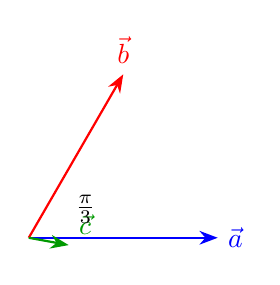
\begin{tikzpicture}[scale=1.2, >=Stealth]
    \draw[->, thick, blue] (0,0,0) -- (2,0,0) node[right] {$\vec{a}$};
    \draw[->, thick, red] (0,0,0) -- (1,1.73,0) node[above] {$\vec{b}$};
    \draw[->, thick, green!60!black] (0,0,0) -- (1,0.5,1.5) node[above right] {$\vec{c}$};
    \node at (0.6,0.3) {$\frac{\pi}{3}$};
\end{tikzpicture}
\end{center}

\textbf{সমাধান:}

দেওয়া আছে, $|\vec{a}| = |\vec{b}| = |\vec{c}| = 1$ এবং প্রতি জোড়ার মধ্যবর্তী কোণ $\frac{\pi}{3}$।
অতএব, $\vec{a} \cdot \vec{b} = \vec{b} \cdot \vec{c} = \vec{c} \cdot \vec{a} = 1 \cdot 1 \cdot \cos\left(\frac{\pi}{3}\right) = \frac{1}{2}$।

প্রদত্ত সমীকরণ:
$$\vec{a} \times \vec{b} + \vec{b} \times \vec{c} = p\vec{a} + q\vec{b} + r\vec{c}$$

১. সমীকরণের উভয় পক্ষে $\vec{a}$ দ্বারা ডট গুণ করে পাই:
$$\vec{a} \cdot (\vec{a} \times \vec{b}) + \vec{a} \cdot (\vec{b} \times \vec{c}) = p(\vec{a} \cdot \vec{a}) + q(\vec{a} \cdot \vec{b}) + r(\vec{a} \cdot \vec{c})$$
$$\Rightarrow 0 + [\vec{a} \ \vec{b} \ \vec{c}] = p(1) + q\left(\frac{1}{2}\right) + r\left(\frac{1}{2}\right)$$
$$\Rightarrow [\vec{a} \ \vec{b} \ \vec{c}] = p + \frac{q}{2} + \frac{r}{2} \quad \text{--- (i)}$$

২. উভয় পক্ষে $\vec{b}$ দ্বারা ডট গুণ করে পাই:
$$\vec{b} \cdot (\vec{a} \times \vec{b}) + \vec{b} \cdot (\vec{b} \times \vec{c}) = p(\vec{b} \cdot \vec{a}) + q(\vec{b} \cdot \vec{b}) + r(\vec{b} \cdot \vec{c})$$
$$\Rightarrow 0 + 0 = p\left(\frac{1}{2}\right) + q(1) + r\left(\frac{1}{2}\right)$$
$$\Rightarrow p + 2q + r = 0 \implies p + r = -2q \quad \text{--- (ii)}$$

৩. উভয় পক্ষে $\vec{c}$ দ্বারা ডট গুণ করে পাই:
$$\vec{c} \cdot (\vec{a} \times \vec{b}) + \vec{c} \cdot (\vec{b} \times \vec{c}) = p(\vec{c} \cdot \vec{a}) + q(\vec{c} \cdot \vec{b}) + r(\vec{c} \cdot \vec{c})$$
$$\Rightarrow [\vec{a} \ \vec{b} \ \vec{c}] + 0 = p\left(\frac{1}{2}\right) + q\left(\frac{1}{2}\right) + r(1)$$
$$\Rightarrow [\vec{a} \ \vec{b} \ \vec{c}] = \frac{p}{2} + \frac{q}{2} + r \quad \text{--- (iii)}$$

সমীকরণ (i) ও (iii) তুলনা করে পাই:
$$p + \frac{q}{2} + \frac{r}{2} = \frac{p}{2} + \frac{q}{2} + r \implies \frac{p}{2} = \frac{r}{2} \implies p = r$$

$p = r$ মানটি সমীকরণ (ii)-এ বসিয়ে পাই:
$$2p + 2q = 0 \implies p = -q \text{ এবং } r = -q$$

নির্ণেয় রাশির মান:
$$\frac{p^2 + 2q^2 + r^2}{q^2} = \frac{(-q)^2 + 2q^2 + (-q)^2}{q^2} = \frac{q^2 + 2q^2 + q^2}{q^2} = \frac{4q^2}{q^2} = 4$$

\textbf{উত্তর:} $4$

\vspace{0.5cm}
\hrule
\vspace{0.5cm}

% ----------------------------------------------------------------------
% Question 35
% ----------------------------------------------------------------------
\subsection*{প্রশ্ন ৩৫}

একজন পুলিশ মোটরসাইকেল চড়ে $30\text{ km/h}$ বেগে একটি চোরকে তাড়া করছে। চোরের গাড়িটি $192\text{ km/h}$ বেগে গতিশীল। পুলিশ চোরকে লক্ষ্য করে তার পিস্তল থেকে $150\text{ m/s}$ বেগে একটি বুলেট ছুড়ল। বুলেটটি কত বেগে চোরের গাড়িকে আঘাত করবে?

\smallskip
\textit{[A policeman riding a motorcycle at $30\text{ km/h}$ is chasing a thief. The thief's car is moving at $192\text{ km/h}$. The policeman fires a bullet at $150\text{ m/s}$ relative to the gun aiming at the thief. With what speed will the bullet hit the thief's car?]}

\vspace{0.3cm}
\begin{center}
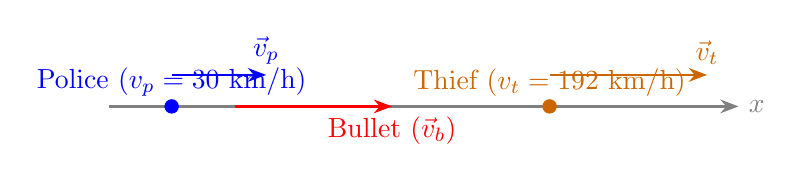
\begin{tikzpicture}[scale=0.8, >=Stealth]
    \draw[->, thick, gray] (0,0) -- (10,0) node[right] {$x$};
    \filldraw[blue] (1,0) circle (3pt) node[above] {Police ($v_p = 30\text{ km/h}$)};
    \draw[->, thick, blue] (1,0.5) -- (2.5,0.5) node[above] {$\vec{v}_p$};
    \draw[->, thick, red] (2,0) -- (4.5,0) node[below] {Bullet ($\vec{v}_b$)};
    \filldraw[orange!80!black] (7,0) circle (3pt) node[above] {Thief ($v_t = 192\text{ km/h}$)};
    \draw[->, thick, orange!80!black] (7,0.5) -- (9.5,0.5) node[above] {$\vec{v}_t$};
\end{tikzpicture}
\end{center}

\textbf{সমাধান:}

এককসমূহকে $\text{m/s}$-এ রূপান্তর করি:
মোটরসাইকেলের (পুলিশের) বেগ, $v_p = 30\text{ km/h} = 30 \times \frac{5}{18} = \frac{25}{3}\text{ m/s}$

চোরের গাড়ির বেগ, $v_t = 192\text{ km/h} = 192 \times \frac{5}{18} = \frac{160}{3}\text{ m/s}$

পিস্তলের সাপেক্ষে বুলেটের আপেক্ষিক বেগ, $v_{bp} = 150\text{ m/s}$

মাটির সাপেক্ষে বুলেটের প্রকৃত বেগ ($v_b$):
$$v_b = v_{bp} + v_p = 150 + \frac{25}{3} = \frac{475}{3}\text{ m/s}$$

চোরের গাড়ির সাপেক্ষে বুলেটের আপেক্ষিক বেগ (যে বেগে আঘাত করবে):
$$v_{bt} = v_b - v_t = \frac{475}{3} - \frac{160}{3} = \frac{315}{3} = 105\text{ m/s}$$

\textbf{উত্তর:} $105\text{ m/s}$

\vspace{0.5cm}
\hrule
\vspace{0.5cm}

% ----------------------------------------------------------------------
% Question 36
% ----------------------------------------------------------------------
\subsection*{প্রশ্ন ৩৬}

একটি নদীতে স্রোতের বেগ $5\text{ km/h}$ এবং একজন সাঁতারুর শান্ত পানিতে সাঁতার কাটার বেগ $3\text{ km/h}$। সাঁতারুটি নদীটি সোজাসুজি (ন্যূনতম দূরত্বে) পার হতে পারবে কি না গাণিতিকভাবে বিশ্লেষণ করো। যদি না পারে, তবে কত কোণে সাঁতার কাটলে তার নদীর পাড় বরাবর বিচ্যুতি (drift) সর্বনিম্ন হবে এবং সেই সর্বনিম্ন বিচ্যুতির মান কত হবে? নদীর প্রস্থ $1\text{ km}$।

\smallskip
\textit{[The river current speed is $5\text{ km/h}$ and a swimmer's speed in still water is $3\text{ km/h}$. Mathematically analyze whether the swimmer can cross the river directly (shortest distance). If not, at what angle should he swim so that his drift along the bank is minimized, and what will be the value of this minimum drift? The width of the river is $1\text{ km}$.]}

\vspace{0.3cm}
\begin{center}
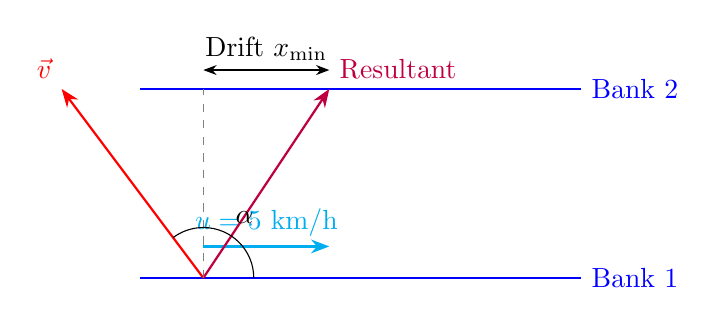
\begin{tikzpicture}[scale=0.8, >=Stealth]
    \draw[thick, blue] (-1,0) -- (6,0) node[right] {Bank 1};
    \draw[thick, blue] (-1,3) -- (6,3) node[right] {Bank 2};
    \draw[->, thick, cyan] (0,0.5) -- (2,0.5) node[midway, above] {$u = 5\text{ km/h}$};
    \draw[->, thick, red] (0,0) -- (126.87:3.75) node[above left] {$\vec{v}$};
    \draw[->, thick, purple] (0,0) -- (2, 3) node[above right] {Resultant};
    \draw[dashed, gray] (0,0) -- (0,3);
    \draw (0,0) ++(0:0.8) arc (0:126.87:0.8) node[midway, above right] {$\alpha$};
    \draw[<->] (0,3.3) -- (2, 3.3) node[midway, above] {Drift $x_{\min}$};
\end{tikzpicture}
\end{center}

\textbf{সমাধান:}

স্রোতের বেগ $u = 5\text{ km/h}$, সাঁতারুর বেগ $v = 3\text{ km/h}$, এবং নদীর প্রস্থ $d = 1\text{ km}$।

যেহেতু $u > v$, সেহেতু সোজাসুজি নদী পার হওয়া অসম্ভব, কারণ $\cos\alpha = -\frac{u}{v} = -\frac{5}{3} < -1$, যা বাস্তবসম্মত নয়।

সর্বনিম্ন বিচ্যুতির ($\text{drift}$) শর্ত:
নদীর পাড় বরাবর বিচ্যুতি $x$:
$$x = (u + v\cos\alpha)t = (u + v\cos\alpha)\frac{d}{v\sin\alpha}$$

বিচ্যুতি $x$ কে সর্বনিম্ন করতে $\frac{dx}{d\alpha} = 0$ হতে হবে, যা থেকে পাওয়া যায়:
$$\cos\alpha = -\frac{v}{u} = -\frac{3}{5} = -0.6 \implies \alpha = \cos^{-1}(-0.6) \approx 126.87^\circ$$

সর্বনিম্ন বিচ্যুতির মান:
যেহেতু $\cos\alpha = -0.6$, সেহেতু $\sin\alpha = \sqrt{1 - (-0.6)^2} = 0.8$।
$$x_{\min} = \frac{d}{v} \left( \frac{u + v\cos\alpha}{\sin\alpha} \right) = \frac{1}{3} \left( \frac{5 + 3(-0.6)}{0.8} \right) = \frac{1}{3} \left( \frac{3.2}{0.8} \right) = \frac{4}{3}\text{ km} \approx 1.33\text{ km}$$

\textbf{উত্তর:} নদীটি সোজাসুজি পার হওয়া সম্ভব নয়। $126.87^\circ$ কোণে সাঁতার কাটলে বিচ্যুতি সর্বনিম্ন $1.33\text{ km}$ হবে।

\vspace{0.5cm}
\hrule
\vspace{0.5cm}

% ----------------------------------------------------------------------
% Question 37
% ----------------------------------------------------------------------
\subsection*{প্রশ্ন ৩৭}

$5\text{ km}$ চওড়া একটি নদীতে স্রোতের বেগ $3\text{ km/h}$ এবং একটি নৌকার নিজস্ব বেগ $4\text{ km/h}$। মাঝি নদীটি সোজাসুজি (ন্যূনতম পথে) পার হওয়ার জন্য নির্দিষ্ট কোণে যাত্রা শুরু করল। কিন্তু যাত্রা শুরুর $1\text{ h}$ পর সে সিদ্ধান্ত পরিবর্তন করে এবং বাকি পথ "সর্বনিম্ন সময়ে নদী পারাপার" এর শর্তে চালনা শুরু করল। নৌকাটির ওপারে পৌঁছাতে সর্বমোট কত সময় লেগেছিল?

\smallskip
\textit{[In a $5\text{ km}$ wide river, the river current speed is $3\text{ km/h}$ and a boat's speed is $4\text{ km/h}$. The boatman started steering at an angle to cross directly along the shortest path. But after $1\text{ h}$, he changed his decision and steered the remaining path under the condition of "shortest time crossing". What was the total time taken for the boat to reach the opposite bank?]}

\vspace{0.3cm}
\begin{center}
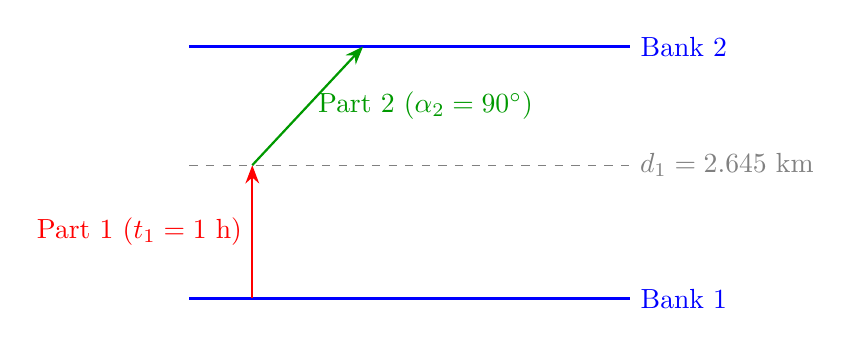
\begin{tikzpicture}[scale=0.8, >=Stealth]
    \draw[thick, blue] (-1,0) -- (6,0) node[right] {Bank 1};
    \draw[thick, blue] (-1,4) -- (6,4) node[right] {Bank 2};
    \draw[dashed, gray] (-1,2.116) -- (6,2.116) node[right] {$d_1 = 2.645\text{ km}$};
    \draw[->, thick, red] (0,0) -- (0,2.116) node[midway, left] {Part 1 ($t_1=1\text{ h}$)};
    \draw[->, thick, green!60!black] (0,2.116) -- (1.76,4) node[midway, right] {Part 2 ($\alpha_2=90^\circ$)};
\end{tikzpicture}
\end{center}

\textbf{সমাধান:}

দেওয়া আছে, $d = 5\text{ km}$, $u = 3\text{ km/h}$, $v = 4\text{ km/h}$।

১ম অংশ (ন্যূনতম পথে পারাপারের চেষ্টা):
সোজাসুজি পার হওয়ার কোণ $\alpha_1$:
$$\cos\alpha_1 = -\frac{u}{v} = -\frac{3}{4} \implies \alpha_1 \approx 138.59^\circ$$

প্রস্থ বরাবর বেগের উপাংশ:
$$v_{y1} = v\sin\alpha_1 = 4\sin(138.59^\circ) \approx 2.645\text{ km/h}$$

$t_1 = 1\text{ h}$ সময়ে প্রস্থ বরাবর অতিক্রান্ত দূরত্ব:
$$d_1 = v_{y1} \times t_1 = 2.645\text{ km}$$

বাকি পথ:
$$d_2 = d - d_1 = 5 - 2.645 = 2.355\text{ km}$$

২য় অংশ (বাকি পথ সর্বনিম্ন সময়ে পারাপার):
সর্বনিম্ন সময়ে নদী পারাপারের জন্য খাড়া সোজাসুজি পাড়ি দিতে হয় ($\alpha_2 = 90^\circ$)। এক্ষেত্রে প্রস্থ বরাবর বেগ $v_{y2} = v = 4\text{ km/h}$।

প্রয়োজনীয় সময়:
$$t_2 = \frac{d_2}{v} = \frac{2.355}{4} \approx 0.588\text{ h}$$

সর্বমোট সময়:
$$t_{\text{total}} = t_1 + t_2 = 1 + 0.588 = 1.588\text{ h}\text{ (বা } 1\text{ ঘণ্টা } 35\text{ মিনিট } 18\text{ সেকেন্ড)}$$

\textbf{উত্তর:} $1.588\text{ h}$ বা $1\text{ ঘণ্টা } 35\text{ মিনিট } 18\text{ সেকেন্ড}$

\vspace{0.5cm}
\hrule
\vspace{0.5cm}

% ----------------------------------------------------------------------
% Question 38
% ----------------------------------------------------------------------
\subsection*{প্রশ্ন ৩৮}

একটি কণা x-অক্ষ বরাবর $x = (10 + 8t + 3t^2)\text{ m}$ এবং অপর একটি কণা y-অক্ষ বরাবর $y = (5 + 3t^3)\text{ m}$ সমীকরণ অনুযায়ী গতিশীল। $t = 1\text{ s}$ সময়ে প্রথম কণার সাপেক্ষে দ্বিতীয় কণার আপেক্ষিক বেগের মান ও দিক নির্ণয় করো।

\smallskip
\textit{[One particle moves along the x-axis according to $x = (10 + 8t + 3t^2)\text{ m}$ and another particle moves along the y-axis according to $y = (5 + 3t^3)\text{ m}$. Find the magnitude and direction of the relative velocity of the second particle with respect to the first particle at $t = 1\text{ s}$.]}

\vspace{0.3cm}
\begin{center}
\begin{tikzpicture}[scale=0.55, >=Stealth]
    \draw[->, gray] (-15,0) -- (4,0) node[right] {$x$};
    \draw[->, gray] (0,-2) -- (0,10) node[above] {$y$};
    \draw[->, thick, blue] (0,0) -- (14,0) node[right] {$\vec{v}_1$};
    \draw[->, thick, red] (0,0) -- (0,9) node[above] {$\vec{v}_2$};
    \draw[->, thick, purple] (0,0) -- (-14,9) node[above left] {$\vec{v}_{21} = \vec{v}_2 - \vec{v}_1$};
    \draw[dashed, gray] (-14,0) -- (-14,9) -- (0,9);
\end{tikzpicture}
\end{center}

\textbf{সমাধান:}

১. প্রথম কণার বেগ ($\vec{v}_1$):
$$v_1 = \frac{dx}{dt} = \frac{d}{dt}(10 + 8t + 3t^2) = 8 + 6t$$
$t = 1\text{ s}$ সময়ে, $v_1 = 8 + 6(1) = 14\text{ m/s} \implies \vec{v}_1 = 14\hat{i}\text{ m/s}$

২. দ্বিতীয় কণার বেগ ($\vec{v}_2$):
$$v_2 = \frac{dy}{dt} = \frac{d}{dt}(5 + 3t^3) = 9t^2$$
$t = 1\text{ s}$ সময়ে, $v_2 = 9(1)^2 = 9\text{ m/s} \implies \vec{v}_2 = 9\hat{j}\text{ m/s}$

৩. ১ম কণার সাপেক্ষে ২য় কণার আপেক্ষিক বেগ ($\vec{v}_{21}$):
$$\vec{v}_{21} = \vec{v}_2 - \vec{v}_1 = -14\hat{i} + 9\hat{j}\text{ m/s}$$

আপেক্ষিক বেগের মান:
$$|\vec{v}_{21}| = \sqrt{(-14)^2 + 9^2} = \sqrt{196 + 81} = \sqrt{277} \approx 16.64\text{ m/s}$$

দিক (x-অক্ষের ঋণাত্মক দিকের সাথে উৎপন্ন কোণ $\theta$):
$$\tan\theta = \frac{9}{14} \implies \theta = \tan^{-1}(0.643) \approx 32.74^\circ\text{ (উত্তর-পশ্চিম দিকে)}$$

\textbf{উত্তর:} আপেক্ষিক বেগের মান $16.64\text{ m/s}$ এবং দিক x-অক্ষের ঋণাত্মক দিকের সাথে $32.74^\circ$ কোণে।

\vspace{0.5cm}
\hrule
\vspace{0.5cm}

% ----------------------------------------------------------------------
% Question 39
% ----------------------------------------------------------------------
\subsection*{প্রশ্ন ৩৯}

একটি নৌকা $u$ বেগে সোজা পূর্ব দিকে গতিশীল। একই সময়ে একটি জাহাজ $2u$ বেগে পূর্ব দিকের সাথে $\theta$ কোণে উত্তর দিকে যাচ্ছে। যদি নৌকার আরোহীর কাছে মনে হয় যে জাহাজটি সোজা উত্তর-পূর্ব দিকে যাচ্ছে, তবে ভেক্টর জ্যামিতির সাহায্যে প্রমাণ করো যে, $\cos\theta - \sin\theta = \frac{1}{2}$।

\smallskip
\textit{[A boat is moving due east at speed $u$. At the same time, a ship is moving at speed $2u$ at an angle $\theta$ north of east. If it appears to a passenger on the boat that the ship is moving directly North-East, prove using vector geometry that $\cos\theta - \sin\theta = \frac{1}{2}$.]}

\vspace{0.3cm}
\begin{center}
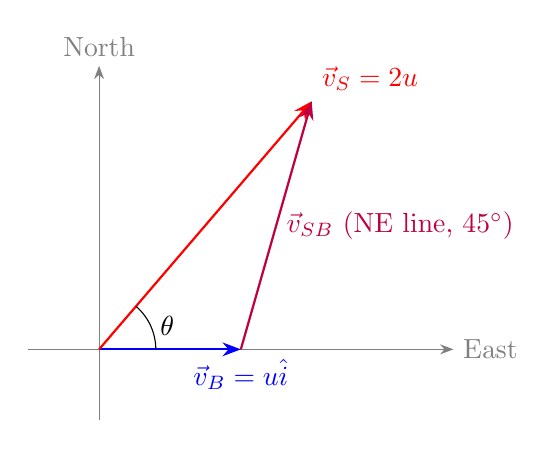
\begin{tikzpicture}[scale=0.9, >=Stealth]
    \draw[->, gray] (-1,0) -- (5,0) node[right] {East};
    \draw[->, gray] (0,-1) -- (0,4) node[above] {North};
    \draw[->, thick, blue] (0,0) -- (2,0) node[below] {$\vec{v}_B = u\hat{i}$};
    \draw[->, thick, red] (0,0) -- (3,3.5) node[above right] {$\vec{v}_S = 2u$};
    \draw[->, thick, purple] (2,0) -- (3,3.5) node[midway, right] {$\vec{v}_{SB}$ (NE line, $45^\circ$)};
    \draw (0.8,0) arc (0:49:0.8) node[midway, right] {$\theta$};
\end{tikzpicture}
\end{center}

\textbf{সমাধান:}

পূর্ব দিককে $\hat{i}$ এবং উত্তর দিককে $\hat{j}$ ধরি।
নৌকার বেগ, $\vec{v}_B = u\hat{i}$
জাহাজের বেগ, $\vec{v}_S = 2u\cos\theta\hat{i} + 2u\sin\theta\hat{j}$

নৌকার সাপেক্ষে জাহাজের আপেক্ষিক বেগ ($\vec{v}_{SB}$):
$$\vec{v}_{SB} = \vec{v}_S - \vec{v}_B = (2u\cos\theta - u)\hat{i} + 2u\sin\theta\hat{j}$$

যেহেতু আপেক্ষিক গতিপথ সোজা উত্তর-পূর্ব (North-East) দিকে (অর্থাৎ $45^\circ$ কোণে), তাই x-উপাংশ এবং y-উপাংশ সমান হতে হবে:
$$2u\cos\theta - u = 2u\sin\theta$$

$u \neq 0$ হওয়ায় উভয় পক্ষকে $u$ দ্বারা ভাগ করে পাই:
$$2\cos\theta - 1 = 2\sin\theta \implies 2\cos\theta - 2\sin\theta = 1$$
$$\Rightarrow \cos\theta - \sin\theta = \frac{1}{2} \quad \text{(প্রমাণিত)}$$

\vspace{0.5cm}
\hrule
\vspace{0.5cm}

% ----------------------------------------------------------------------
% Question 40
% ----------------------------------------------------------------------
\subsection*{প্রশ্ন ৪০}

একটি স্থির নৌকার উপর টাঙানো পতাকা উত্তর-পশ্চিম মাঝামাঝি দিক বরাবর $71\text{ km/h}$ বেগে উড়ছে। নৌকাটি হঠাৎ $51\text{ km/h}$ বেগে উত্তর দিকে চলতে শুরু করলে পতাকাটি কত বেগে এবং কোন দিকে উড়বে?

\smallskip
\textit{[A flag hoisted on a stationary boat is fluttering in the North-West direction at a speed of $71\text{ km/h}$. If the boat suddenly starts moving North at $51\text{ km/h}$, at what speed and in which direction will the flag flutter?]}

\vspace{0.3cm}
\begin{center}
\begin{tikzpicture}[scale=0.7, >=Stealth]
    \draw[->, gray] (-4,0) -- (4,0) node[right] {E};
    \draw[->, gray] (0,-4) -- (0,4) node[above] {N};
    \draw[->, thick, cyan] (0,0) -- (-3.53,3.53) node[above left] {$\vec{v}_w$ (NW)};
    \draw[->, thick, blue] (0,0) -- (0,3.6) node[right] {$\vec{v}_b$ (North)};
    \draw[->, thick, red] (0,0) -- (-3.53,-0.06) node[below left] {$\vec{v}_{wb}$};
\end{tikzpicture}
\end{center}

\textbf{সমাধান:}

পূর্ব দিককে $+x$ এবং উত্তর দিককে $+y$ অক্ষ ধরি।
স্থির নৌকায় পতাকাটি বাতাসের প্রকৃত বেগে উড়বে। উত্তর-পশ্চিম দিক বরাবর (অনূভূমিকের সাথে $135^\circ$ কোণে) বাতাসের বেগ:
$$\vec{v}_w = 71\cos 135^\circ\hat{i} + 71\sin 135^\circ\hat{j} \approx -50.2\hat{i} + 50.2\hat{j}\text{ km/h}$$

চলমান নৌকার বেগ, $\vec{v}_b = 51\hat{j}\text{ km/h}$।

নৌকার সাপেক্ষে বাতাসের আপেক্ষিক বেগ (পতাকা ওড়ার দিক), $\vec{v}_{wb}$:
$$\vec{v}_{wb} = \vec{v}_w - \vec{v}_b = (-50.2\hat{i} + 50.2\hat{j}) - 51\hat{j} = -50.2\hat{i} - 0.8\hat{j}\text{ km/h}$$

পতাকা ওড়ার বেগ:
$$|\vec{v}_{wb}| = \sqrt{(-50.2)^2 + (-0.8)^2} \approx 50.21\text{ km/h}$$

দিক (দক্ষিণ দিকের সাথে উৎপন্ন কোণ $\theta$):
$$\tan\theta = \frac{|v_x|}{|v_y|} = \frac{50.2}{0.8} = 62.75 \implies \theta \approx 89.09^\circ\text{ (পশ্চিম দিকে)}$$

\textbf{উত্তর:} পতাকাটি $50.21\text{ km/h}$ বেগে দক্ষিণ দিক হতে $89.09^\circ$ পশ্চিমে উড়বে।

\vspace{0.5cm}
\hrule
\vspace{0.5cm}

% ----------------------------------------------------------------------
% Question 41
% ----------------------------------------------------------------------
\subsection*{প্রশ্ন ৪১}

খাড়া নিচের দিকে $5\text{ m/s}$ বেগে বৃষ্টি পড়ছে। হঠাৎ পূর্ব থেকে পশ্চিম দিকে $2\text{ m/s}$ বেগে বাতাস বইতে শুরু করল।
(ক) স্থির দাঁড়িয়ে থাকা একটি পূর্বমুখী গাড়ির সামনের ও পিছনের কাচের কোনটি ভিজবে এবং কত কোণে ভিজবে?
(খ) গাড়িটি যদি $3\text{ m/s}$ বেগে পূর্ব দিকে চলতে শুরু করে, তবে গাড়ির কাচ ভেজার উপর এর কী প্রভাব পড়বে গাণিতিক বিশ্লেষণ সহ দেখাও।

\smallskip
\textit{[Rain is falling vertically downward at $5\text{ m/s}$. Suddenly wind starts blowing from East to West at $2\text{ m/s}$. (a) Which glass (front or rear) of a stationary East-facing car will get wet and at what angle? (b) If the car starts moving East at $3\text{ m/s}$, mathematically analyze the effect on which glass gets wet.]}

\vspace{0.3cm}
\begin{center}
\begin{tikzpicture}[scale=0.7, >=Stealth]
    \draw[->, gray] (-4,0) -- (4,0) node[right] {East};
    \draw[->, gray] (0,-4) -- (0,2) node[above] {Vertical};
    \draw[->, thick, cyan] (0,0) -- (-2,0) node[above] {Wind $\vec{v}_w$};
    \draw[->, thick, blue] (0,0) -- (0,-5) node[right] {Rain $\vec{v}_r$};
    \draw[->, thick, red] (0,0) -- (-2,-5) node[below left] {Resultant Rain};
    \draw[dashed, gray] (-2,0) -- (-2,-5) -- (0,-5);
\end{tikzpicture}
\end{center}

\textbf{সমাধান:}

পূর্ব দিককে $+x$ এবং খাড়া উপরের দিককে $+y$ অক্ষ ধরি।
বৃষ্টির বেগ $\vec{v}_r = -5\hat{j}$, বাতাসের বেগ $\vec{v}_w = -2\hat{i}$।
বৃষ্টির মোট প্রকৃত বেগ, $\vec{v}_{\text{rain}} = -2\hat{i} - 5\hat{j}$।

(ক) স্থির পূর্বমুখী গাড়ির ক্ষেত্রে:
গাড়ির সাপেক্ষে বৃষ্টির বেগ $\vec{v}_{\text{rel}} = -2\hat{i} - 5\hat{j}$।
যেহেতু x-উপাংশ ঋণাত্মক (পশ্চিমমুখী), বৃষ্টি সামনের দিক থেকে আসবে। ফলে সামনের কাচ ভিজবে।
কোণ:
$$\tan\theta = \frac{|v_x|}{|v_y|} = \frac{2}{5} = 0.4 \implies \theta = \tan^{-1}(0.4) \approx 21.8^\circ\text{ (উল্লম্বের সাথে)}$$

(খ) গাড়িটি $3\text{ m/s}$ বেগে পূর্ব দিকে গতিশীল হলে:
গাড়ির বেগ $\vec{v}_c = 3\hat{i}$।
আপেক্ষিক বেগ:
$$\vec{v}_{\text{rel}}' = \vec{v}_{\text{rain}} - \vec{v}_c = (-2\hat{i} - 5\hat{j}) - 3\hat{i} = -5\hat{i} - 5\hat{j}$$
এখানেও x-উপাংশ ঋণাত্মক হওয়ায় সামনের কাচই ভিজবে, তবে নতুন কোণ হবে:
$$\tan\theta' = \frac{5}{5} = 1 \implies \theta' = 45^\circ\text{ (উল্লম্বের সাথে)}$$

\textbf{উত্তর:} (ক) সামনের কাচ $21.8^\circ$ কোণে ভিজবে। (খ) গাড়ি পূর্ব দিকে চললে বৃষ্টি $45^\circ$ কোণে সামনের কাচকে ভিজিয়ে দেবে।

\vspace{0.5cm}
\hrule
\vspace{0.5cm}

% ----------------------------------------------------------------------
% Question 42
% ----------------------------------------------------------------------
\subsection*{প্রশ্ন ৪২}

কোনো আরোহী $5\text{ m/s}$ বেগে দৌড়ালে বৃষ্টি তার গায়ে লম্বভাবে পড়ে। আরোহী তার বেগ দ্বিগুণ করলে বৃষ্টি উল্লম্ব রেখার সাথে $30^\circ$ কোণে বেঁকে পড়ে। বৃষ্টির প্রকৃত বেগ ও দিক নির্ণয় করো।

\smallskip
\textit{[When a runner runs at $5\text{ m/s}$, rain appears to fall vertically on him. When he doubles his speed, rain appears to fall inclined at $30^\circ$ to the vertical. Find the actual velocity and direction of the rain.]}

\vspace{0.3cm}
\begin{center}
\begin{tikzpicture}[scale=0.7, >=Stealth]
    \draw[->, gray] (-1,0) -- (6,0) node[right] {$x$};
    \draw[->, gray] (0,-6) -- (0,1) node[above] {$y$};
    \draw[->, thick, blue] (0,0) -- (3,0) node[above] {$v_1 = 5$};
    \draw[->, thick, red] (0,0) -- (3,-5.196) node[below right] {$\vec{v}_r$};
    \draw[->, thick, green!50!black] (0,0) -- (0,-5.196) node[left] {$\vec{v}_{r1}$ (vertical)};
    \draw[dashed, gray] (3,0) -- (3,-5.196);
\end{tikzpicture}
\end{center}

\textbf{সমাধান:}

ধরি, বৃষ্টির প্রকৃত বেগ $\vec{v}_r = v_x\hat{i} + v_y\hat{j}$।

১ম ক্ষেত্র ($v_1 = 5\text{ m/s}$):
বৃষ্টি লম্বভাবে পড়ার শর্তে অনুভূমিক আপেক্ষিক বেগ শূন্য:
$$v_x - 5 = 0 \implies v_x = 5\text{ m/s}$$

২য় ক্ষেত্র ($v_2 = 10\text{ m/s}$):
আপেক্ষিক বেগ উল্লম্বের সাথে $30^\circ$ কোণ তৈরি করে:
$$\tan 30^\circ = \frac{|v_x - 10|}{|v_y|} \implies \frac{1}{\sqrt{3}} = \frac{|5 - 10|}{|v_y|} = \frac{5}{|v_y|}$$
$$\Rightarrow |v_y| = 5\sqrt{3}\text{ m/s} \implies v_y = -5\sqrt{3}\text{ m/s}$$

বৃষ্টির প্রকৃত বেগের মান:
$$|\vec{v}_r| = \sqrt{5^2 + (-5\sqrt{3})^2} = \sqrt{25 + 75} = \sqrt{100} = 10\text{ m/s}$$

দিক (উল্লম্বের সাথে):
$$\tan\theta = \frac{v_x}{|v_y|} = \frac{5}{5\sqrt{3}} = \frac{1}{\sqrt{3}} \implies \theta = 30^\circ$$

\textbf{উত্তর:} বৃষ্টির প্রকৃত বেগ $10\text{ m/s}$ এবং এটি উল্লম্বের সাথে $30^\circ$ কোণে হেলে পড়ছে।

\vspace{0.5cm}
\hrule
\vspace{0.5cm}

% ----------------------------------------------------------------------
% Question 43
% ----------------------------------------------------------------------
\subsection*{প্রশ্ন ৪৩}

ধরি, ত্রিমাত্রিক কার্তেসীয় তলে $\vec{p}, \vec{q}$ এবং $\vec{r}$ তিনটি অসমতলীয় ভেক্টর। একটি ভেক্টর $\vec{s}$ এর উপাংশত্রয় $\vec{p}, \vec{q}$ এবং $\vec{r}$ বরাবর যথাক্রমে $4, 3$ এবং $5$। যদি এই একই ভেক্টর $\vec{s}$ এর উপাংশত্রয় তিনটি নতুন অক্ষ যথাক্রমে $(-\vec{p}+\vec{q}+\vec{r})$, $(\vec{p}-\vec{q}+\vec{r})$ এবং $(-\vec{p}-\vec{q}+\vec{r})$ বরাবর যথাক্রমে $x, y$ এবং $z$ হয়, তবে $2x+y+z$ এর মান নির্ণয় করো।

\smallskip
\textit{[Let $\vec{p}, \vec{q},$ and $\vec{r}$ be three non-coplanar vectors in 3D Cartesian space. The components of a vector $\vec{s}$ along $\vec{p}, \vec{q},$ and $\vec{r}$ are $4, 3,$ and $5$ respectively. If the components of the same vector $\vec{s}$ along three new axes $(-\vec{p}+\vec{q}+\vec{r})$, $(\vec{p}-\vec{q}+\vec{r})$, and $(-\vec{p}-\vec{q}+\vec{r})$ are $x, y,$ and $z$ respectively, find the value of $2x+y+z$.]}

\vspace{0.3cm}
\begin{center}
\begin{tikzpicture}[scale=1.0, >=Stealth]
    \draw[->, thick, blue] (0,0,0) -- (2,0,0) node[right] {$\vec{p}$};
    \draw[->, thick, blue] (0,0,0) -- (0,2,0) node[above] {$\vec{q}$};
    \draw[->, thick, blue] (0,0,0) -- (0,0,2) node[below left] {$\vec{r}$};
    \draw[->, thick, red] (0,0,0) -- (1.5,1.5,1.5) node[above right] {$\vec{s}$};
\end{tikzpicture}
\end{center}

\textbf{সমাধান:}

প্রশ্নানুসারে, ভেক্টর $\vec{s}$ কে আদি ও নতুন দুই জোড়া অক্ষের সাহায্যে প্রকাশ করে পাই:
$$\vec{s} = 4\vec{p} + 3\vec{q} + 5\vec{r} \quad \text{--- (i)}$$
এবং
$$\vec{s} = x(-\vec{p} + \vec{q} + \vec{r}) + y(\vec{p} - \vec{q} + \vec{r}) + z(-\vec{p} - \vec{q} + \vec{r})$$
$$\Rightarrow \vec{s} = (-x + y - z)\vec{p} + (x - y - z)\vec{q} + (x + y + z)\vec{r} \quad \text{--- (ii)}$$

$\vec{p}, \vec{q}, \vec{r}$ অসমতলীয় হওয়ায় সহগসমূহ তুলনা করে পাই:
$$-x + y - z = 4 \quad \text{--- (1)}$$
$$x - y - z = 3 \quad \text{--- (2)}$$
$$x + y + z = 5 \quad \text{--- (3)}$$

সমীকরণ (2) ও (3) যোগ করে পাই:
$$2x = 8 \implies x = 4$$

সমীকরণ (1) ও (3) যোগ করে পাই:
$$2y = 9 \implies y = 4.5$$

$x$ ও $y$ এর মান (3)-এ বসিয়ে পাই:
$$4 + 4.5 + z = 5 \implies z = -3.5$$

নির্ণেয় রাশির মান:
$$2x + y + z = 2(4) + 4.5 + (-3.5) = 8 + 4.5 - 3.5 = 9$$

\textbf{উত্তর:} $9$

\vspace{0.5cm}
\hrule
\vspace{0.5cm}

% ----------------------------------------------------------------------
% Question 44
% ----------------------------------------------------------------------
\subsection*{প্রশ্ন ৪৪}

একজন আরোহী $10\text{ km/h}$ বেগে দৌড়ে যাওয়ার সময় বৃষ্টির ফোঁটা তার গায়ে খাড়া লম্বভাবে $5\text{ km/h}$ বেগে পড়তে দেখল। বৃষ্টির প্রকৃত বেগের মান ও দিক নির্ণয় করো।

\smallskip
\textit{[While running at $10\text{ km/h}$, a runner sees raindrops falling vertically on him at $5\text{ km/h}$. Find the magnitude and direction of the actual velocity of rain.]}

\vspace{0.3cm}
\begin{center}
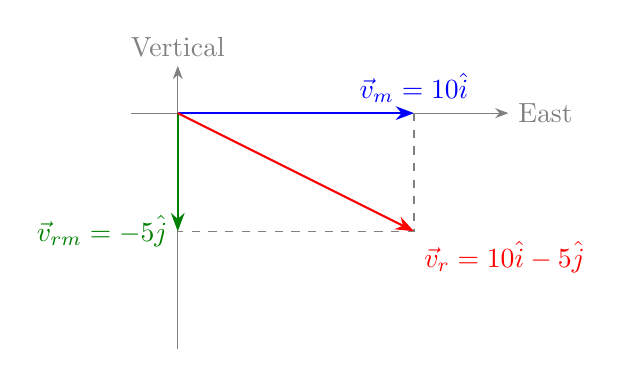
\begin{tikzpicture}[scale=0.6, >=Stealth]
    \draw[->, gray] (-1,0) -- (7,0) node[right] {East};
    \draw[->, gray] (0,-5) -- (0,1) node[above] {Vertical};
    \draw[->, thick, blue] (0,0) -- (5,0) node[above] {$\vec{v}_m = 10\hat{i}$};
    \draw[->, thick, green!50!black] (0,0) -- (0,-2.5) node[left] {$\vec{v}_{rm} = -5\hat{j}$};
    \draw[->, thick, red] (0,0) -- (5,-2.5) node[below right] {$\vec{v}_r = 10\hat{i}-5\hat{j}$};
    \draw[dashed, gray] (5,0) -- (5,-2.5) -- (0,-2.5);
\end{tikzpicture}
\end{center}

\textbf{সমাধান:}

আরোহীর বেগ $\vec{v}_m = 10\hat{i}\text{ km/h}$ এবং আপেক্ষিক বেগ $\vec{v}_{rm} = -5\hat{j}\text{ km/h}$।

আমরা জানি:
$$\vec{v}_{rm} = \vec{v}_r - \vec{v}_m \implies \vec{v}_r = \vec{v}_{rm} + \vec{v}_m = 10\hat{i} - 5\hat{j}\text{ km/h}$$

বৃষ্টির প্রকৃত বেগের মান:
$$|\vec{v}_r| = \sqrt{10^2 + (-5)^2} = \sqrt{125} = 5\sqrt{5}\text{ km/h} \approx 11.18\text{ km/h}$$

দিক (উল্লম্বের সাথে কোণ $\theta$):
$$\tan\theta = \frac{|v_{rx}|}{|v_{ry}|} = \frac{10}{5} = 2 \implies \theta = \tan^{-1}(2) \approx 63.43^\circ$$

\textbf{উত্তর:} বৃষ্টির প্রকৃত বেগ $11.18\text{ km/h}$ এবং এটি উল্লম্বের সাথে $63.43^\circ$ কোণে হেলে আরোহীর গতির অভিমুখে পড়ছে।

\vspace{0.5cm}
\hrule
\vspace{0.5cm}

% ----------------------------------------------------------------------
% Question 45
% ----------------------------------------------------------------------
\subsection*{প্রশ্ন ৪৫}

যদি $\vec{b}$, $\vec{c}$ এবং $\vec{d}$ তিনটি অসমতলীয় (non-coplanar) ভেক্টর হয়, তবে ভেক্টর বীজগণিতের সূত্রাবলী ব্যবহার করে প্রমাণ করো যে, $(\vec{a} \times \vec{b}) \times (\vec{c} \times \vec{d}) + (\vec{a} \times \vec{c}) \times (\vec{d} \times \vec{b}) + (\vec{a} \times \vec{d}) \times (\vec{b} \times \vec{c})$ ভেক্টরটি সর্বদা $\vec{a}$ ভেক্টরের সমান্তরাল।

\smallskip
\textit{[If $\vec{b}$, $\vec{c}$, and $\vec{d}$ are three non-coplanar vectors, prove using vector algebra identities that the vector $(\vec{a} \times \vec{b}) \times (\vec{c} \times \vec{d}) + (\vec{a} \times \vec{c}) \times (\vec{d} \times \vec{b}) + (\vec{a} \times \vec{d}) \times (\vec{b} \times \vec{c})$ is always parallel to $\vec{a}$.]}

\vspace{0.3cm}
\begin{center}
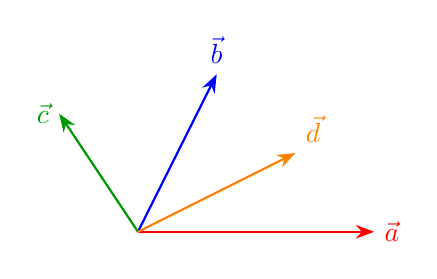
\begin{tikzpicture}[scale=1.0, >=Stealth]
    \draw[->, thick, red] (0,0) -- (3,0) node[right] {$\vec{a}$};
    \draw[->, thick, blue] (0,0) -- (1,2) node[above] {$\vec{b}$};
    \draw[->, thick, green!60!black] (0,0) -- (-1,1.5) node[left] {$\vec{c}$};
    \draw[->, thick, orange] (0,0) -- (2,1) node[above right] {$\vec{d}$};
\end{tikzpicture}
\end{center}

\textbf{সমাধান:}

ধরি, লব্ধি ভেক্টরটি $\vec{V}$। ভেক্টর ত্রয়ী গুণন সূত্র প্রয়োগ করে প্রতিটি পদ বিস্তৃত করি:
১. $\vec{T}_1 = (\vec{a} \times \vec{b}) \times (\vec{c} \times \vec{d}) = [\vec{a} \ \vec{c} \ \vec{d}]\vec{b} - [\vec{b} \ \vec{c} \ \vec{d}]\vec{a}$
২. $\vec{T}_2 = (\vec{a} \times \vec{c}) \times (\vec{d} \times \vec{b}) = [\vec{a} \ \vec{d} \ \vec{b}]\vec{c} - [\vec{c} \ \vec{d} \ \vec{b}]\vec{a}$
৩. $\vec{T}_3 = (\vec{a} \times \vec{d}) \times (\vec{b} \times \vec{c}) = [\vec{a} \ \vec{b} \ \vec{c}]\vec{d} - [\vec{d} \ \vec{b} \ \vec{c}]\vec{a}$

সমষ্টি নিয়ে পাই:
$$\vec{V} = \left( [\vec{a} \ \vec{c} \ \vec{d}]\vec{b} + [\vec{a} \ \vec{d} \ \vec{b}]\vec{c} + [\vec{a} \ \vec{b} \ \vec{c}]\vec{d} \right) - \left( [\vec{b} \ \vec{c} \ \vec{d}] + [\vec{c} \ \vec{d} \ \vec{b}] + [\vec{d} \ \vec{b} \ \vec{c}] \right)\vec{a}$$

ভেক্টর অভেদানুসারে:
$$[\vec{a} \ \vec{c} \ \vec{d}]\vec{b} + [\vec{a} \ \vec{d} \ \vec{b}]\vec{c} + [\vec{a} \ \vec{b} \ \vec{c}]\vec{d} = [\vec{b} \ \vec{c} \ \vec{d}]\vec{a}$$

এবং স্কেলার ত্রয়ী গুণফলের চাকার নিয়ম থেকে:
$$[\vec{b} \ \vec{c} \ \vec{d}] = [\vec{c} \ \vec{d} \ \vec{b}] = [\vec{d} \ \vec{b} \ \vec{c}]$$

সুতরাং:
$$\vec{V} = [\vec{b} \ \vec{c} \ \vec{d}]\vec{a} - 3[\vec{b} \ \vec{c} \ \vec{d}]\vec{a} = -2[\vec{b} \ \vec{c} \ \vec{d}]\vec{a}$$

যেহেতু $-2[\vec{b} \ \vec{c} \ \vec{d}]$ একটি বাস্তব স্কেলার, সেহেতু $\vec{V}$ ভেক্টরটি সর্বদা $\vec{a}$ এর সমান্তরাল। (প্রমাণিত)

\vspace{0.5cm}
\hrule
\vspace{0.5cm}

% ----------------------------------------------------------------------
% Question 46
% ----------------------------------------------------------------------
\subsection*{প্রশ্ন ৪৬}

$\lambda$ এর এমন সকল বাস্তব মান নির্ণয় করো যেন নিম্নের ভেক্টর সমীকরণটির একটি অশূন্য বাস্তব সমাধান $(x, y, z) \neq (0, 0, 0)$ বিদ্যমান থাকে:
$$(\hat{i}+\hat{j}+3\hat{k})x + (3\hat{i}-3\hat{j}+\hat{k})y + (-4\hat{i}+5\hat{j})z = \lambda(x\hat{i}+y\hat{j}+z\hat{k})$$

\smallskip
\textit{[Find all real values of $\lambda$ such that the following vector equation has a non-zero real solution $(x, y, z) \neq (0, 0, 0)$: $(\hat{i}+\hat{j}+3\hat{k})x + (3\hat{i}-3\hat{j}+\hat{k})y + (-4\hat{i}+5\hat{j})z = \lambda(x\hat{i}+y\hat{j}+z\hat{k})$.]}

\vspace{0.3cm}
\begin{center}
\begin{tikzpicture}[scale=0.8, >=Stealth]
    \draw[->, thick] (0,0,0) -- (3,0,0) node[right] {$\hat{i}$};
    \draw[->, thick] (0,0,0) -- (0,3,0) node[above] {$\hat{j}$};
    \draw[->, thick] (0,0,0) -- (0,0,3) node[below left] {$\hat{k}$};
    \node at (2,1.5,1) {$\det(D) = 0$};
\end{tikzpicture}
\end{center}

\textbf{সমাধান:}

উভয় পক্ষ হতে $\hat{i}, \hat{j}, \hat{k}$ এর সহগ সমীকৃত করে পাই:
$$(1-\lambda)x + 3y - 4z = 0$$
$$x - (3+\lambda)y + 5z = 0$$
$$3x + y - \lambda z = 0$$

সমজাতীয় রৈখিক সমীকরণ জোটের অশূন্য (non-trivial) সমাধান থাকার শর্তানুসারে নির্ণায়ক শূন্য হবে:
$$D = \begin{vmatrix} 1-\lambda & 3 & -4 \\ 1 & -(3+\lambda) & 5 \\ 3 & 1 & -\lambda \end{vmatrix} = 0$$

বিস্তৃত করে পাই:
$$(1-\lambda) [\lambda(3+\lambda) - 5] - 3 [-\lambda - 15] - 4 [1 + 3(3+\lambda)] = 0$$
$$\Rightarrow (1-\lambda) (\lambda^2 + 3\lambda - 5) + 3(\lambda + 15) - 4(3\lambda + 10) = 0$$
$$\Rightarrow -\lambda^3 - 2\lambda^2 - \lambda = 0 \implies -\lambda(\lambda + 1)^2 = 0$$

অতএব, $\lambda = 0$ অথবা $\lambda = -1$।

\textbf{উত্তর:} $\lambda = 0, -1$

\vspace{0.5cm}
\hrule
\vspace{0.5cm}

% ----------------------------------------------------------------------
% Question 47
% ----------------------------------------------------------------------
\subsection*{প্রশ্ন ৪৭}

কোনো ত্রিভুজ $\Delta PQR$ এর তিনটি বাহুর দিক বরাবর ক্রমিক ভেক্টর যথাক্রমে $\vec{a} = \vec{QR}$, $\vec{b} = \vec{RP}$ এবং $\vec{c} = \vec{PQ}$। যদি $|\vec{a}| = 12$, $|\vec{b}| = 4\sqrt{3}$ এবং $\vec{b} \cdot \vec{c} = 24$ হয়, তবে প্রমাণ করো যে, $\vec{a} \cdot \vec{b} = -72$ এবং $|\vec{c}|$ এর মান নির্ণয় করো।

\smallskip
\textit{[For a triangle $\Delta PQR$, the vectors along its sides in order are $\vec{a} = \vec{QR}$, $\vec{b} = \vec{RP}$, and $\vec{c} = \vec{PQ}$. If $|\vec{a}| = 12$, $|\vec{b}| = 4\sqrt{3}$, and $\vec{b} \cdot \vec{c} = 24$, prove that $\vec{a} \cdot \vec{b} = -72$ and find the value of $|\vec{c}|$.]}

\vspace{0.3cm}
\begin{center}
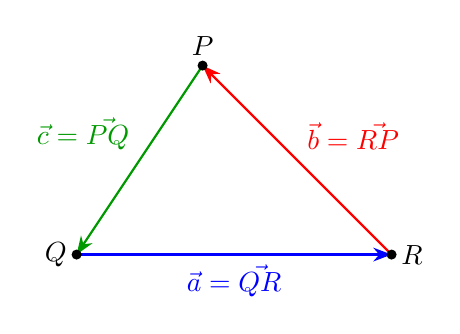
\begin{tikzpicture}[scale=0.8, >=Stealth]
    \coordinate (Q) at (0,0);
    \coordinate (R) at (5,0);
    \coordinate (P) at (2,3);
    \draw[->, thick, blue] (Q) -- (R) node[midway, below] {$\vec{a} = \vec{QR}$};
    \draw[->, thick, red] (R) -- (P) node[midway, above right] {$\vec{b} = \vec{RP}$};
    \draw[->, thick, green!60!black] (P) -- (Q) node[midway, above left] {$\vec{c} = \vec{PQ}$};
    \filldraw (Q) circle (2pt) node[left] {$Q$};
    \filldraw (R) circle (2pt) node[right] {$R$};
    \filldraw (P) circle (2pt) node[above] {$P$};
\end{tikzpicture}
\end{center}

\textbf{সমাধান:}

ত্রিভুজ সূত্রানুসারে:
$$\vec{a} + \vec{b} + \vec{c} = \vec{0} \implies \vec{c} = -(\vec{a} + \vec{b}) \quad \text{--- (i)}$$

১. $\vec{a} \cdot \vec{b} = -72$ প্রমাণ:
দেওয়া আছে $\vec{b} \cdot \vec{c} = 24$:
$$\vec{b} \cdot [-(\vec{a} + \vec{b})] = 24 \implies -\vec{a} \cdot \vec{b} - |\vec{b}|^2 = 24$$
$|\vec{b}| = 4\sqrt{3} \implies |\vec{b}|^2 = 48$ বসিয়ে পাই:
$$-\vec{a} \cdot \vec{b} - 48 = 24 \implies \vec{a} \cdot \vec{b} = -72 \quad \text{(প্রমাণিত)}$$

২. $|\vec{c}|$ এর মান নির্ণয়:
$$|\vec{c}|^2 = [-(\vec{a} + \vec{b})] \cdot [-(\vec{a} + \vec{b})] = |\vec{a}|^2 + |\vec{b}|^2 + 2(\vec{a} \cdot \vec{b})$$
$$|\vec{c}|^2 = 12^2 + 48 + 2(-72) = 144 + 48 - 144 = 48$$
$$\Rightarrow |\vec{c}| = \sqrt{48} = 4\sqrt{3}$$

\textbf{উত্তর:} $|\vec{c}| = 4\sqrt{3}$

\end{document}